
\begin{figure}[ht]
  \centering
  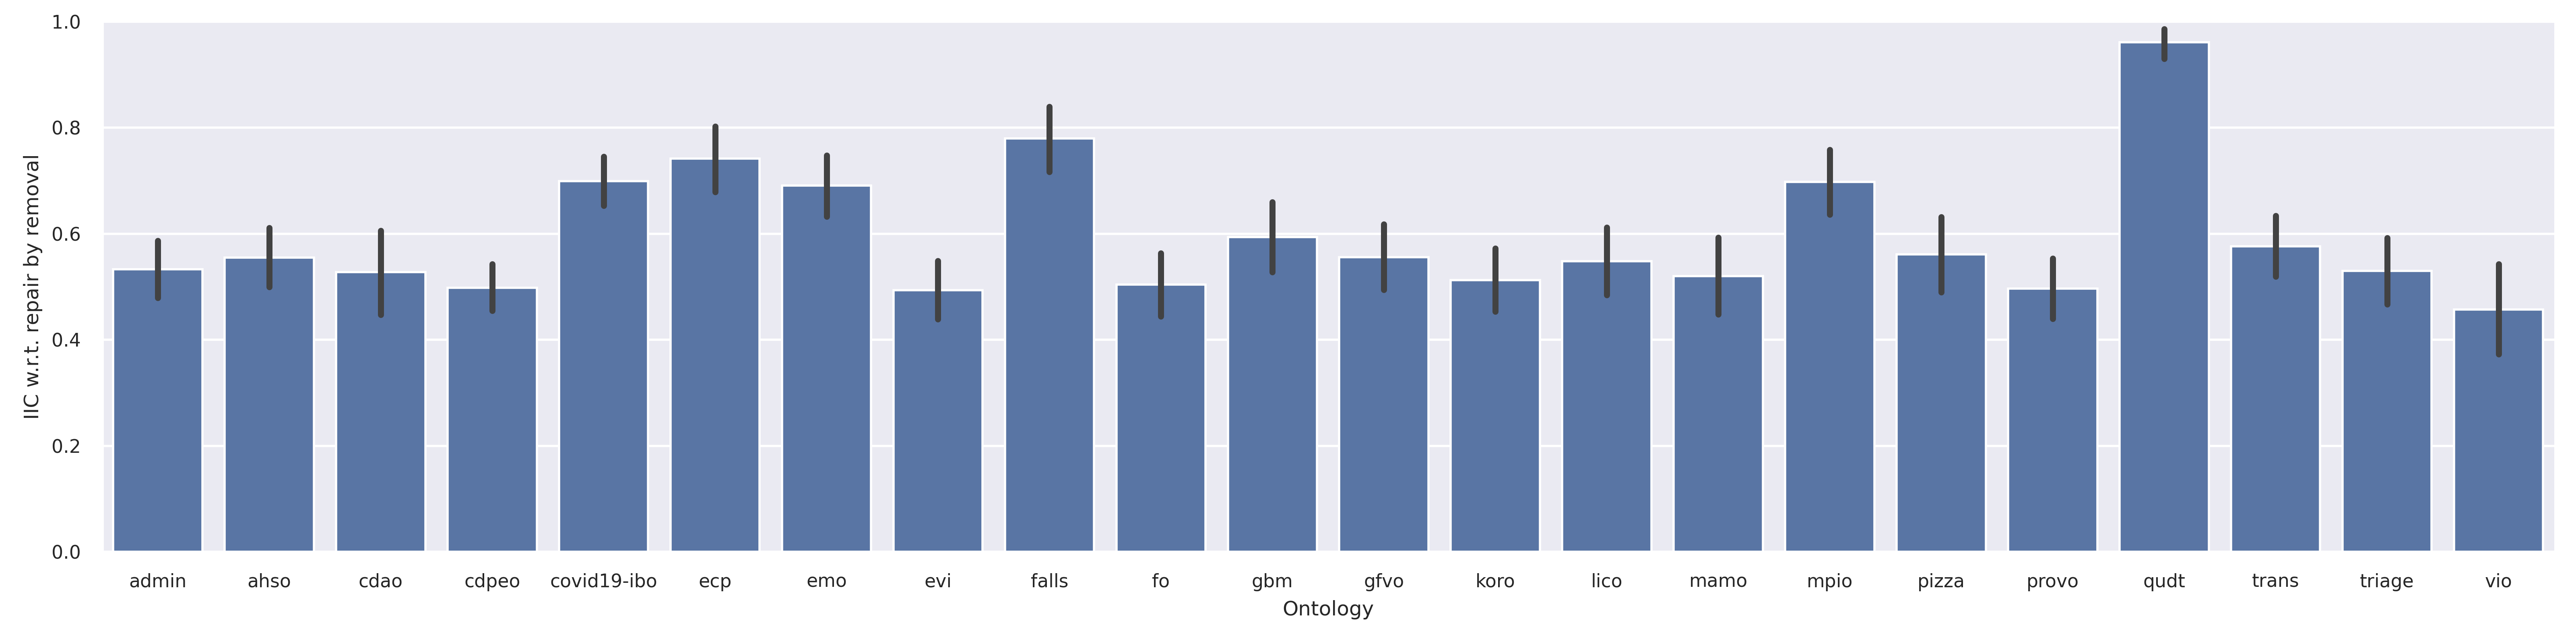
\includegraphics[width=\textwidth]{resources/iic-remove-ontology-bar.png}
  \caption{Mean IIC of weakening based repair with respect to repair via removal per ontology. The error bars show the 95\% confidence interval.}
\end{figure}

\begin{figure}[ht]
  \centering
  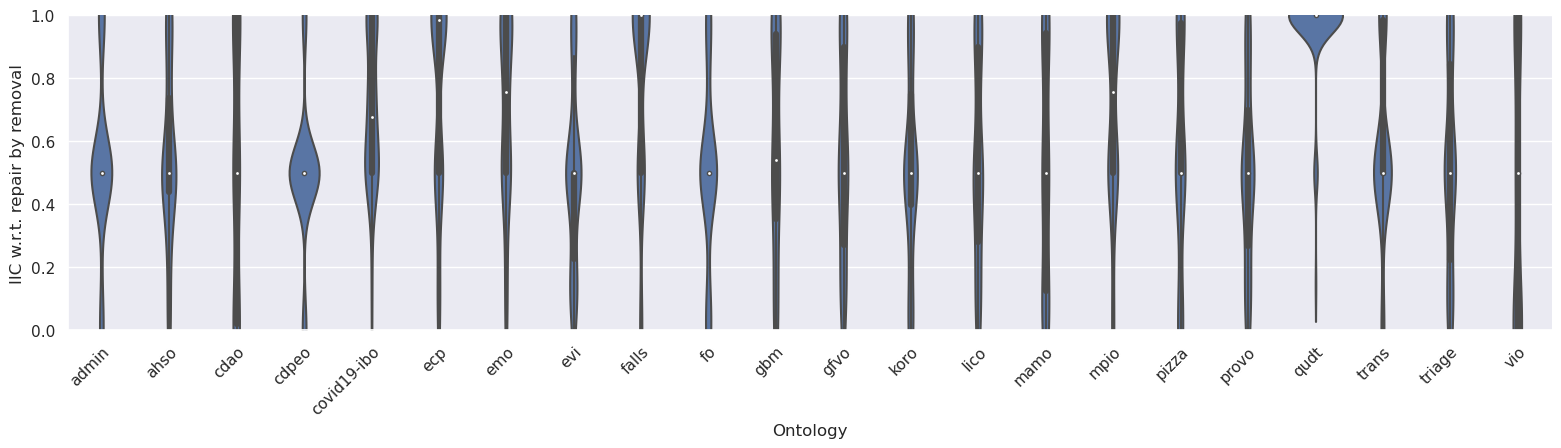
\includegraphics[width=\textwidth]{resources/iic-remove-ontology-violin.png}
  \caption{Distribution of IIC of weakening based repair with respect to repair via removal per ontology.}
\end{figure}

\begin{figure}[ht]
  \centering
  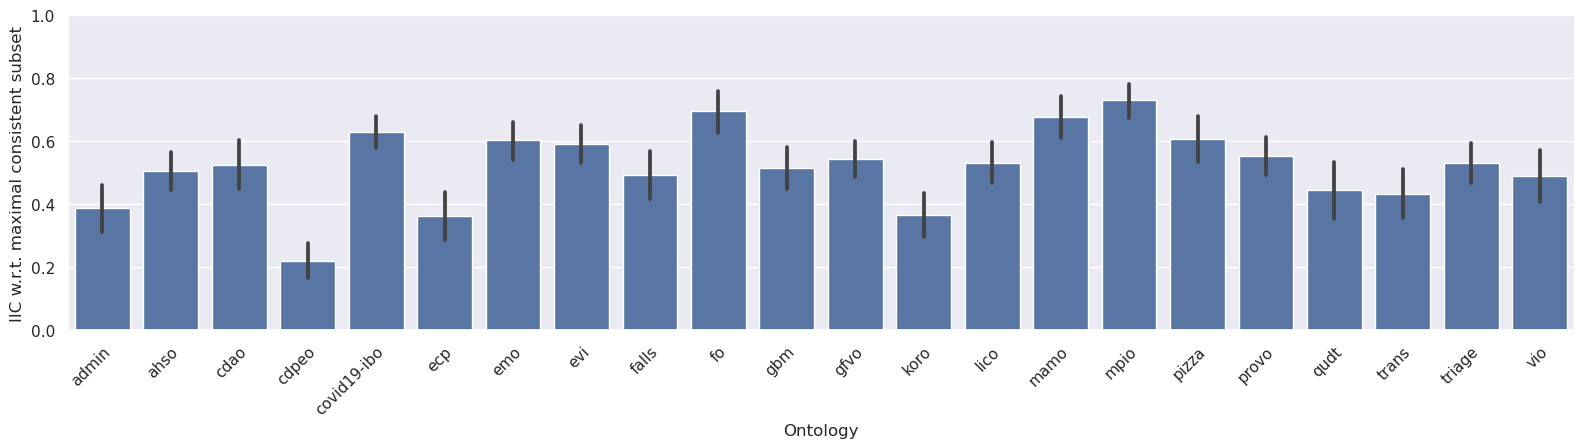
\includegraphics[width=\textwidth]{resources/iic-mcs-ontology-bar.png}
  \caption{Mean IIC of weakening based repair with respect to repair via a random maximal consistent subset per ontology. The error bars show the 95\% confidence interval.}
\end{figure}

\begin{figure}[ht]
    \centering
    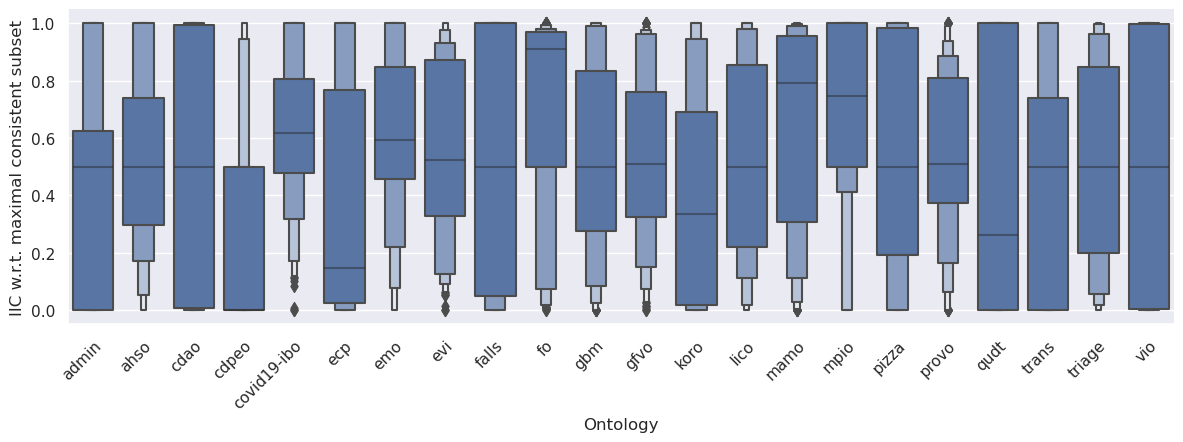
\includegraphics[width=\textwidth]{resources/iic-mcs-ontology-violin.png}
    \caption{Distribution of IIC of weakening based repair with respect to repair via a random maximal consistent subset per ontology.}
\end{figure}

\begin{figure}[ht]
  \centering
  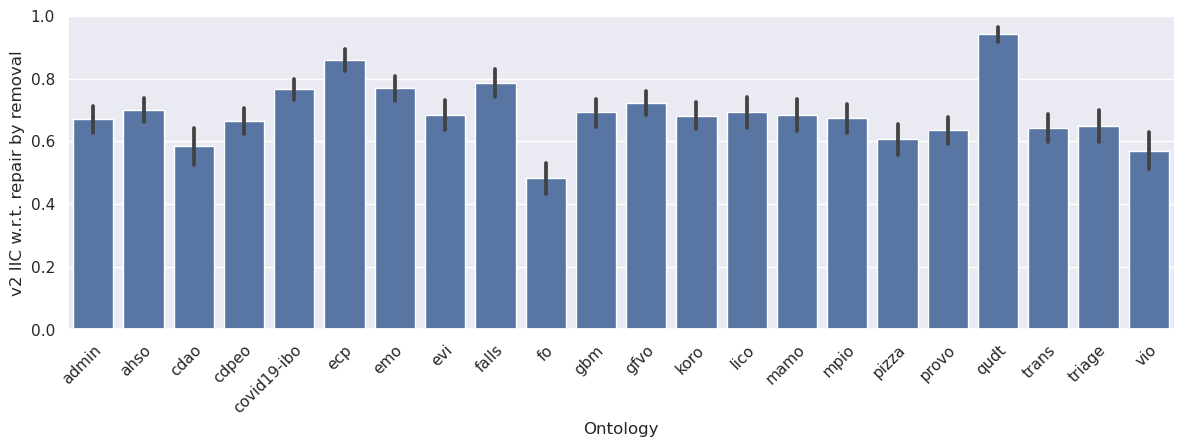
\includegraphics[width=\textwidth]{resources/iic-enhance-rem-ontology-bar.png}
  \caption{Mean IIC of weakening based repair (without weakening axioms in the reference ontology) with respect to repair via removal per ontology. The error bars show the 95\% confidence interval.}
\end{figure}

\begin{figure}[ht]
  \centering
  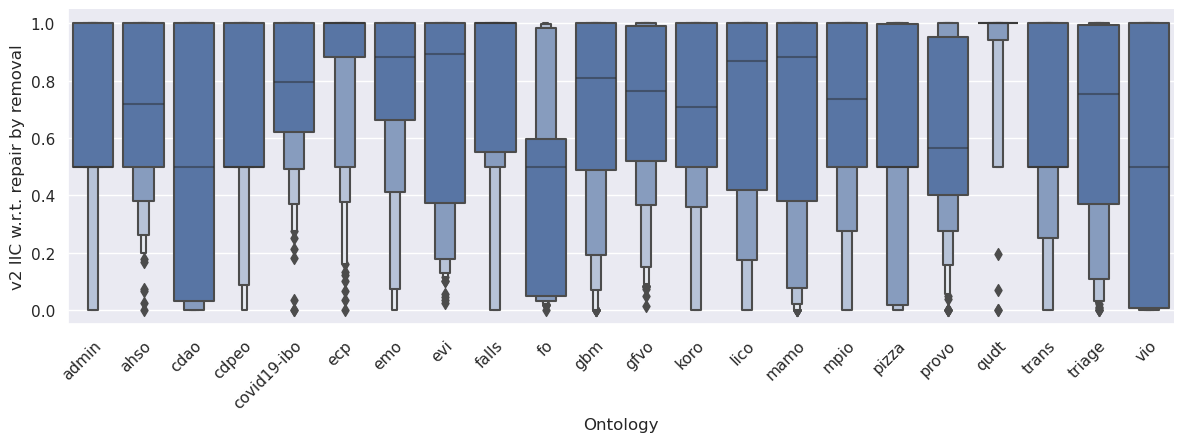
\includegraphics[width=\textwidth]{resources/iic-enhance-rem-ontology-violin.png}
  \caption{Distribution of IIC of weakening based repair (without weakening axioms in the reference ontology) with respect to repair via removal per ontology.}
\end{figure}

\begin{figure}[ht]
  \centering
  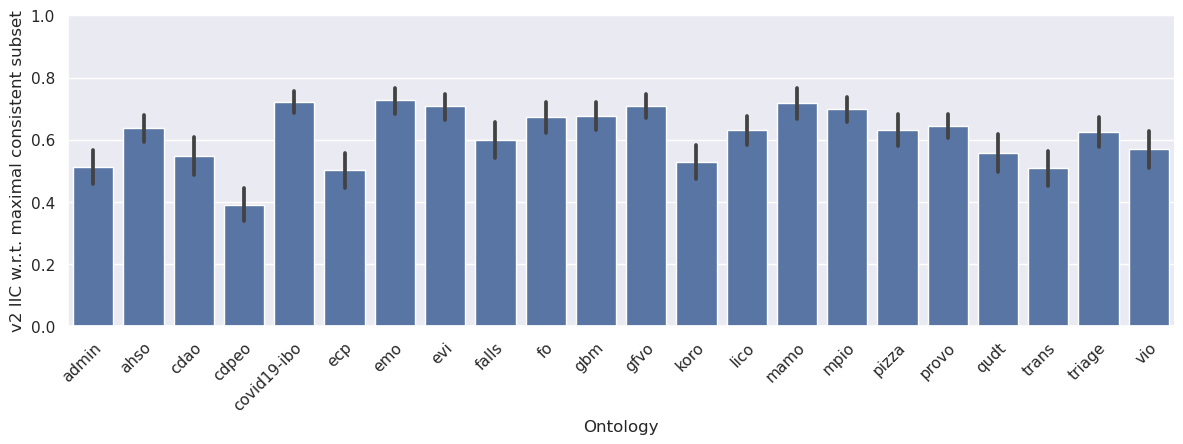
\includegraphics[width=\textwidth]{resources/iic-enhance-ontology-bar.png}
  \caption{Mean IIC of weakening based repair (without weakening axioms in the reference ontology) with respect to repair via a random maximal consistent subset per ontology. The error bars show the 95\% confidence interval.}
\end{figure}

\begin{figure}[ht]
    \centering
    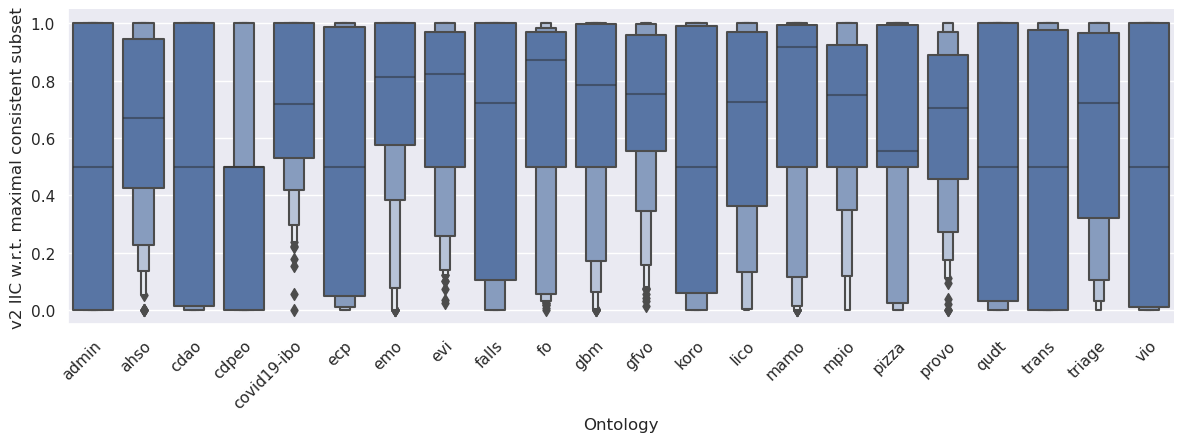
\includegraphics[width=\textwidth]{resources/iic-enhance-ontology-violin.png}
    \caption{Distribution of IIC of weakening based repair (without weakening axioms in the reference ontology) with respect to repair via a random maximal consistent subset per ontology.}
\end{figure}

\begin{figure}[ht]
  \centering
  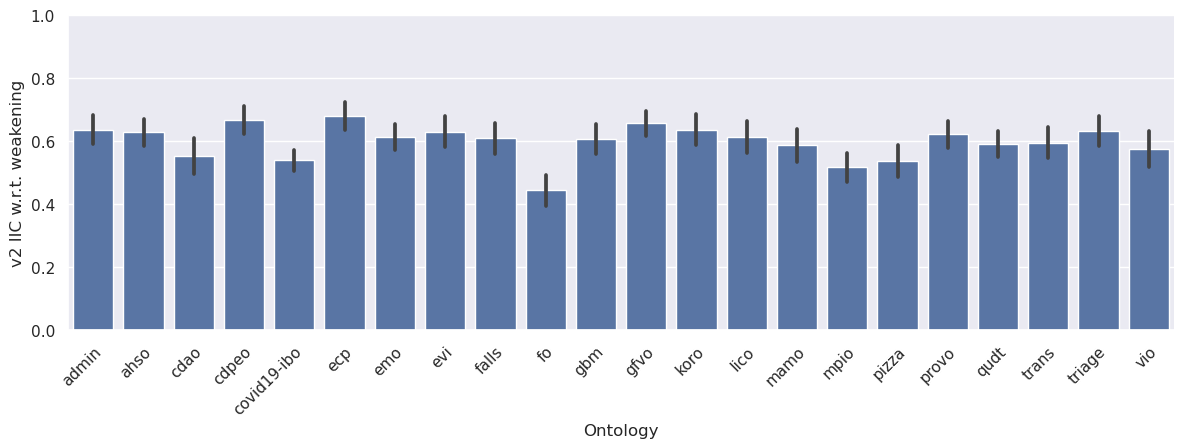
\includegraphics[width=\textwidth]{resources/iic-enhance-weaken-ontology-bar.png}
  \caption{Mean IIC of weakening based repair (without weakening axioms in the reference ontology) with respect to normal repair using axiom weakening per ontology. The error bars show the 95\% confidence interval.}
\end{figure}

\begin{figure}[ht]
    \centering
    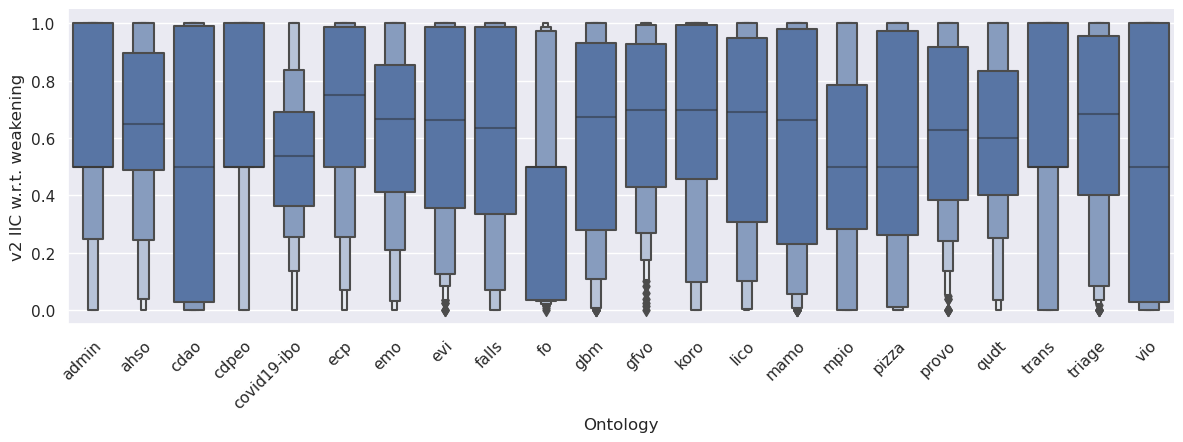
\includegraphics[width=\textwidth]{resources/iic-enhance-weaken-ontology-violin.png}
    \caption{Distribution of IIC of weakening based repair (without weakening axioms in the reference ontology) with respect to normal repair using axiom weakening per ontology.}
\end{figure}

\begin{figure}[ht]
  \centering
  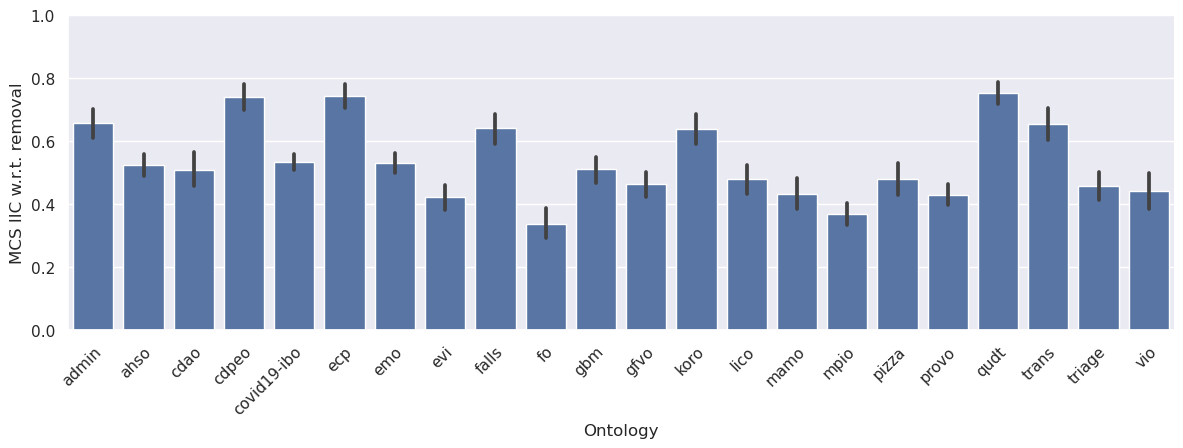
\includegraphics[width=\textwidth]{resources/iic-mcs-rem-ontology-bar.png}
  \caption{Mean IIC of repair using a random maximal consistent subset with respect to repair using removal. The error bars show the 95\% confidence interval.}
\end{figure}

\begin{figure}[ht]
    \centering
    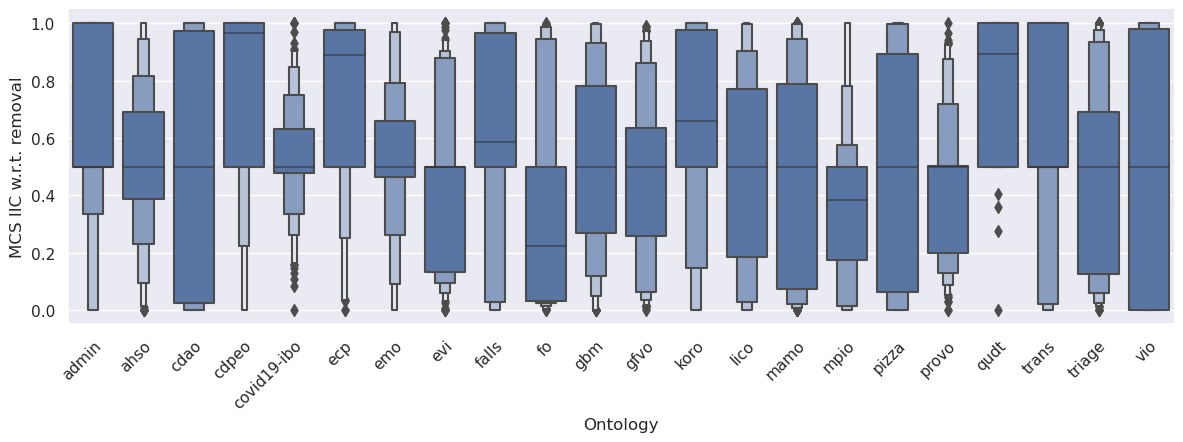
\includegraphics[width=\textwidth]{resources/iic-mcs-rem-ontology-violin.png}
    \caption{Distribution of IIC of repair using random maximal consistent subset with respect to repair using removal per ontology.}
\end{figure}

\begin{table}[ht]
  \scriptsize
  \begin{widepage}
    \centering
    \begin{tabular}{|l|cccccc|}
      \cline{2-7}
      \multicolumn{1}{r|}{IIC of} & \multicolumn{3}{c}{Weakening adding to reference ontology} & \multicolumn{2}{c}{Weakening} & MCS \\
      \multicolumn{1}{r|}{w.r.t.} & Weakening & MCS & Removal & MCS & Removal & Removal \\
      \hline
      admin & 0.64 [0.59, 0.69] & 0.51 [0.45, 0.57] & 0.67 [0.62, 0.72] & 0.39 [0.33, 0.45] & 0.56 [0.51, 0.60] & 0.66 [0.61, 0.71] \\
      ahso & 0.63 [0.58, 0.68] & 0.64 [0.59, 0.69] & 0.70 [0.66, 0.74] & 0.52 [0.47, 0.56] & 0.57 [0.52, 0.62] & 0.52 [0.48, 0.56] \\
      cdao & 0.55 [0.49, 0.61] & 0.55 [0.48, 0.61] & 0.58 [0.52, 0.65] & 0.51 [0.44, 0.57] & 0.54 [0.49, 0.61] & 0.51 [0.45, 0.57] \\
      cdpeo & 0.67 [0.62, 0.72] & 0.39 [0.33, 0.45] & 0.66 [0.62, 0.71] & 0.25 [0.20, 0.30] & 0.50 [0.47, 0.53] & 0.74 [0.69, 0.79] \\
      covid19-ibo & 0.54 [0.50, 0.58] & 0.72 [0.68, 0.76] & 0.77 [0.73, 0.81] & 0.62 [0.58, 0.66] & 0.71 [0.67, 0.75] & 0.53 [0.50, 0.56] \\
      ecp & 0.68 [0.63, 0.73] & 0.50 [0.44, 0.56] & 0.86 [0.82, 0.90] & 0.36 [0.30, 0.42] & 0.75 [0.70, 0.80] & 0.74 [0.70, 0.79] \\
      emo & 0.61 [0.57, 0.66] & 0.73 [0.68, 0.77] & 0.77 [0.72, 0.81] & 0.61 [0.56, 0.65] & 0.68 [0.63, 0.72] & 0.53 [0.49, 0.57] \\
      evi & 0.63 [0.58, 0.68] & 0.71 [0.66, 0.75] & 0.68 [0.63, 0.74] & 0.58 [0.53, 0.63] & 0.51 [0.46, 0.55] & 0.42 [0.38, 0.47] \\
      falls & 0.61 [0.56, 0.66] & 0.60 [0.54, 0.66] & 0.79 [0.73, 0.84] & 0.50 [0.44, 0.57] & 0.75 [0.70, 0.81] & 0.64 [0.59, 0.69] \\
      fo & 0.44 [0.39, 0.50] & 0.67 [0.62, 0.73] & 0.48 [0.43, 0.54] & 0.68 [0.63, 0.73] & 0.53 [0.48, 0.58] & 0.34 [0.29, 0.39] \\
      gbm & 0.61 [0.55, 0.66] & 0.68 [0.63, 0.73] & 0.69 [0.64, 0.74] & 0.54 [0.49, 0.59] & 0.59 [0.54, 0.64] & 0.51 [0.46, 0.56] \\
      gfvo & 0.66 [0.61, 0.70] & 0.71 [0.67, 0.75] & 0.72 [0.68, 0.77] & 0.54 [0.49, 0.59] & 0.53 [0.47, 0.58] & 0.46 [0.42, 0.51] \\
      koro & 0.64 [0.58, 0.69] & 0.53 [0.47, 0.59] & 0.68 [0.63, 0.73] & 0.38 [0.32, 0.43] & 0.53 [0.48, 0.58] & 0.64 [0.59, 0.69] \\
      lico & 0.61 [0.56, 0.67] & 0.63 [0.58, 0.68] & 0.69 [0.64, 0.75] & 0.51 [0.46, 0.57] & 0.53 [0.48, 0.59] & 0.48 [0.43, 0.53] \\
      mamo & 0.59 [0.53, 0.64] & 0.72 [0.66, 0.77] & 0.68 [0.63, 0.74] & 0.64 [0.58, 0.69] & 0.55 [0.49, 0.61] & 0.43 [0.38, 0.49] \\
      mpio & 0.52 [0.46, 0.57] & 0.70 [0.65, 0.74] & 0.67 [0.62, 0.72] & 0.70 [0.66, 0.75] & 0.69 [0.65, 0.74] & 0.37 [0.33, 0.41] \\
      pizza & 0.54 [0.48, 0.59] & 0.63 [0.58, 0.69] & 0.61 [0.55, 0.66] & 0.57 [0.51, 0.63] & 0.56 [0.51, 0.62] & 0.48 [0.42, 0.53] \\
      provo & 0.62 [0.57, 0.67] & 0.64 [0.60, 0.69] & 0.64 [0.59, 0.68] & 0.55 [0.51, 0.60] & 0.51 [0.47, 0.56] & 0.43 [0.39, 0.47] \\
      qudt & 0.59 [0.55, 0.64] & 0.56 [0.49, 0.62] & 0.94 [0.91, 0.97] & 0.47 [0.40, 0.53] & 0.96 [0.93, 0.98] & 0.75 [0.71, 0.79] \\
      trans & 0.60 [0.54, 0.65] & 0.51 [0.45, 0.57] & 0.64 [0.59, 0.69] & 0.41 [0.35, 0.47] & 0.56 [0.51, 0.61] & 0.65 [0.60, 0.71] \\
      triage & 0.63 [0.58, 0.69] & 0.63 [0.57, 0.68] & 0.65 [0.59, 0.71] & 0.52 [0.47, 0.57] & 0.51 [0.46, 0.56] & 0.46 [0.41, 0.51] \\
      vio & 0.58 [0.51, 0.64] & 0.57 [0.51, 0.63] & 0.57 [0.51, 0.63] & 0.50 [0.44, 0.57] & 0.48 [0.41, 0.54] & 0.44 [0.38, 0.50]\\
      \hline
      Overall & 0.60 [0.58, 0.61] & 0.61 [0.60, 0.63] & 0.69 [0.67, 0.70] & 0.52 [0.50, 0.53] & 0.60 [0.58, 0.61] & 0.53 [0.52, 0.55] \\
      \hline
    \end{tabular}
  \end{widepage}
  \caption{Results of the evaluation. IIC is given as mean and 95\% confidence interval in brackets.}
\end{table}

\begin{table}[ht]
  \scriptsize
  \centering
  \begin{tabular}{|l|r@{ }lr@{ }lr@{ }lr@{ }l|}
    \cline{2-9}
    \multicolumn{1}{r|}{$|\Inf(\Omc)|$ of} & \multicolumn{2}{c}{Weakening$^a$} & \multicolumn{2}{c}{Weakening} & \multicolumn{2}{c}{MCS} & \multicolumn{2}{c|}{Removal} \\
    \hline
    admin & 290 & [265, 317] & 255 & [237, 274] & 318 & [287, 352] & 218 & [211, 226] \\
    ahso & 757 & [730, 784] & 704 & [680, 728]& 717 & [691, 743] & 712 & [685, 738] \\
    cdao & 2843 & [2494, 3202] & 2592 & [2317, 2889] & 2841 & [2529, 3178] & 2637 & [2364, 2937] \\
    cdpeo & 179 & [176, 183] & 171 & [169, 173] & 193 & [187, 199] & 171 & [169, 173] \\
    covid19-ibo & 6832 & [6499, 7155] & 6696 & [6364, 7001] & 6517 & [6185, 6839] & 6362 & [6028, 6673] \\
    ecp & 345 & [320, 370] & 271 & [256, 286] & 412 & [384, 441] & 260 & [247, 274] \\
    emo & 6625 & [6328, 6925] & 6318 & [6027, 6622] & 6115 & [5830, 6420] & 6055 & [5763, 6353] \\
    evi & 785 & [764, 804] & 766 & [745, 786] & 736 & [714, 756] & 771 & [750, 792] \\
    falls & 248 & [232, 265] & 234 & [219, 251] & 247 & [232, 263] & 225 & [211, 240] \\
    fo & 979 & [959, 997] & 980 & [957, 1001] & 924 & [900, 947] & 964 & [936, 989] \\
    gbm & 6062 & [5850, 6269] & 5796 & [5577, 6007] & 5827 & [5621, 6020] & 5687 & [5463, 5910] \\
    gfvo & 8766 & [8613, 8907] & 8202 & [8018, 8373] & 7940 & [7733, 8133] & 8126 & [7925, 8319] \\
    koro & 1243 & [1156, 1343] & 1015 & [986, 1046] & 1311 & [1214, 1419] & 991 & [967, 1017] \\
    lico & 6532 & [6284, 6766] & 6150 & [5870, 6417] & 6251 & [5996, 6504] & 6166 & [5881, 6433] \\
    mamo & 9071 & [8647, 9462] & 8945 & [8558, 9304] & 8208 & [7812, 8591] & 8422 & [7974, 8858] \\
    mpio & 479 & [458, 500] & 483 & [462, 503] & 413 & [395, 430] & 465 & [446, 484] \\
    pizza & 6694 & [6268, 7102] & 6437 & [6071, 6814] & 6404 & [6046, 6759] & 6077 & [5695, 6461] \\
    provo & 759 & [742, 774] & 737 & [720, 753] & 714 & [695, 733] & 738 & [721, 754] \\
    qudt & 560 & [508, 617] & 539 & [491, 594] & 613 & [549, 686] & 524 & [478, 578] \\
    trans & 408 & [389, 428] & 379 & [369, 390] & 441 & [413, 471] & 363 & [355, 371] \\
    triage & 775 & [742, 808] & 727 & [695, 759] & 743 & [712, 773] & 750 & [717, 784] \\
    vio & 2264 & [2009, 2530] & 2074 & [1814, 2337] & 2017 & [1788, 2255] & 2087 & [1826, 2362] \\
    \hline
  \end{tabular}
  \caption{Results of the evaluation. The cardinality of the inferred class hierarchy is given as mean and 95\% confidence interval in brackets. $^a$Weakening based repair that keeps the reference ontology as static axioms that are not weakened or replaced.}
\end{table}

% TODO: add extended quality for weakening w.r.t mcs (2 figures)
% TODO: add extended quality for weakening w.r.t remove (2 figures)
% TODO: add extended quality for enhance w.r.t mcs (2 figures)
% TODO: add extended quality for enhance w.r.t remove (2 figures)
% TODO: add extended quality for enhance w.r.t weakening (2 figures)
% TODO: add extended quality for mcs w.r.t remove (2 figures)
% TODO: add extended complete quality table
% TODO: add extended table with sizes of inferred set

\begin{figure}[ht]
    \centering
    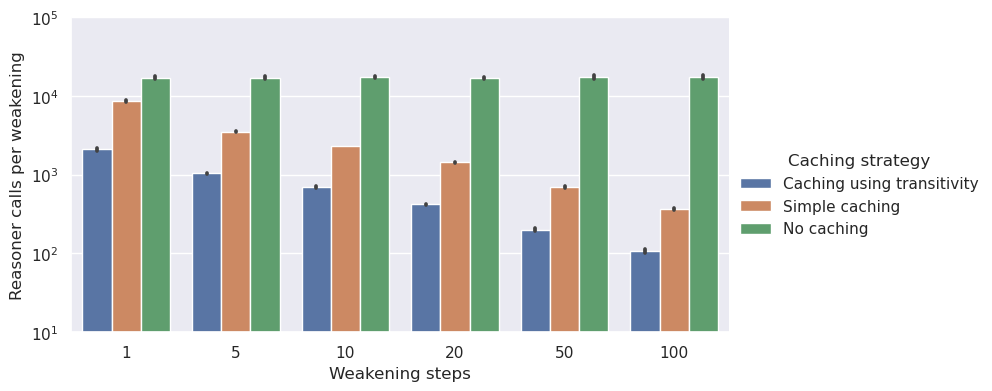
\includegraphics[width=\textwidth]{resources/calls-cache-bar.png}
    \caption{Average reasoner calls with different caching strategies when executing axiom weakening of random axioms. Results are the average between the following ontologies: admin, cdpeo, emo, gbm, gfvo, koro, and mamo. Each consistency or entailment query made to the reasoner count as one call.}
\end{figure}

\begin{figure}[ht]
    \centering
    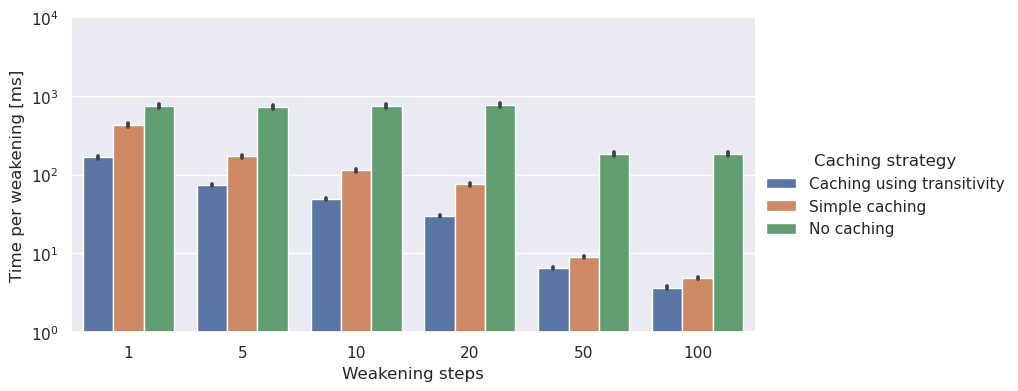
\includegraphics[width=\textwidth]{resources/time-cache-bar.png}
    \caption{Average time required per application of the axiom weakening operator with different caching strategies when executing axiom weakening of random axioms. Results are the average between the following ontologies: admin, cdpeo, emo, gbm, gfvo, koro, and mamo. The results are averaged for the reasoners FaCT++, JFact, Openllet, and HermiT.}
\end{figure}

\begin{figure}[ht]
    \centering
    
\includegraphics[height=0.9\textheight]{resources/calls-cache-ontology-bar.png}
    \caption{Average reasoner calls with different caching strategies when executing axiom weakening of random axioms per ontology. Each consistency or entailment query made to the reasoner count as one call.}
\end{figure}

\begin{figure}[ht]
    \begin{widepage}[3cm]
      \centering
      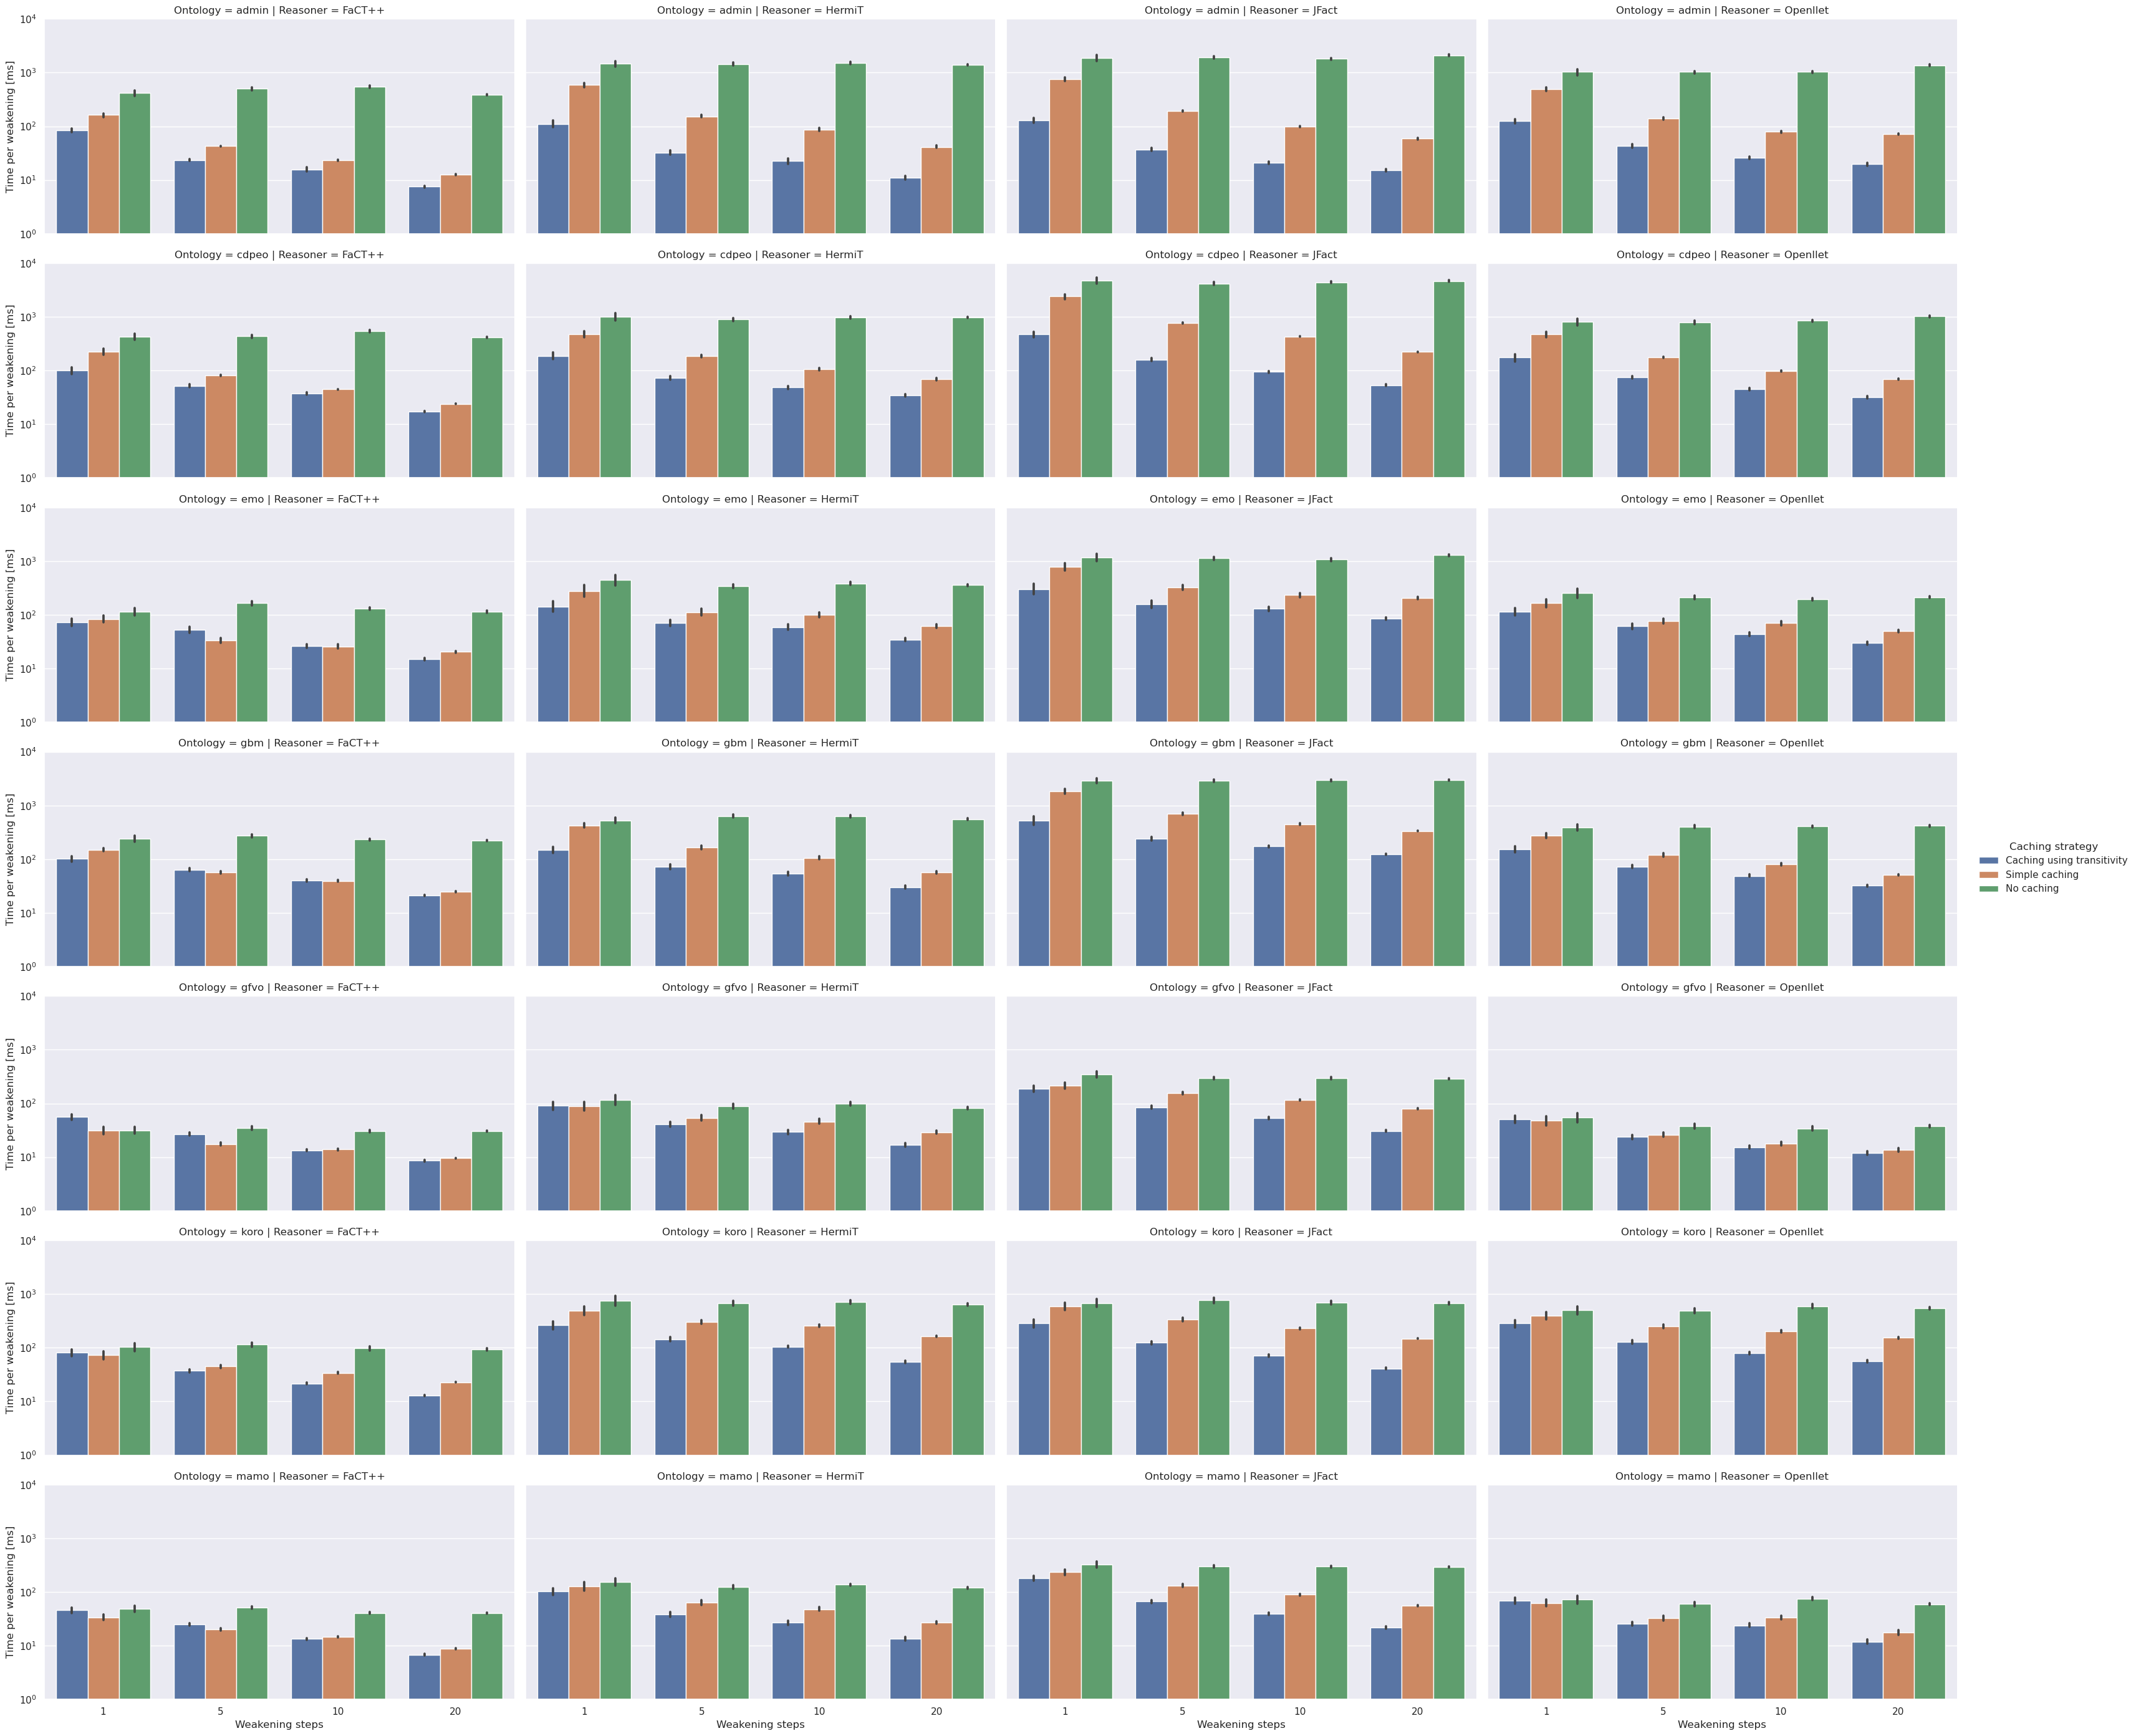
\includegraphics[width=\textwidth]{resources/time-cache-ontology-reasoner-bar.png}
    \end{widepage}
    \caption{Average time required per application of the axiom weakening operator with different caching strategies when executing axiom weakening of random axioms per ontology and reasoner.}
\end{figure}

\begin{table}[ht]
  \scriptsize
  \begin{widepage}[5cm]
    \centering
    \addtolength{\tabcolsep}{-1mm}
    \begin{tabular}{|l|rrrrrr|rrrrrr|rrrrrr|}
      \cline{2-19}
      \multicolumn{1}{l|}{} & \multicolumn{18}{c|}{\hspace{-9mm}Reasoner calls per weakening} \\
      \multicolumn{1}{l|}{} & \multicolumn{6}{c}{Caching using transitivity} & \multicolumn{6}{c}{Simple caching} & \multicolumn{6}{c|}{No caching} \\
      \multicolumn{1}{l|}{} & \multicolumn{1}{c}{1} & \multicolumn{1}{c}{5} & \multicolumn{1}{c}{10} & \multicolumn{1}{c}{20} & \multicolumn{1}{c}{50} & \multicolumn{1}{c}{100} & \multicolumn{1}{c}{1} & \multicolumn{1}{c}{5} & \multicolumn{1}{c}{10} & \multicolumn{1}{c}{20} & \multicolumn{1}{c}{50} & \multicolumn{1}{c}{100} & \multicolumn{1}{c}{1} & \multicolumn{1}{c}{5} & \multicolumn{1}{c}{10} & \multicolumn{1}{c}{20} & \multicolumn{1}{c}{50} & 100 \\
      \hline
      admin & 1096 & 381 & 222 & 131 & 64 & 35
        & 15138 & 4072 & 2115 & 1092 & 459 & 236
        & 41105 & 42224 & 41288 & 41376 & 42663 & 41751 \\
      cdpeo & 2110 & 869 & 522 & 301 & 136 & 75
        & 13621 & 4936 & 2694 & 1436 & 608 & 312
        & 29051 & 27289 & 28617 & 28818 & 28244 & 29315 \\
      emo & 2652 & 1720 & 1355 & 864 & 463 & 258
        & 7781 & 3436 & 2784 & 2023 & 1103 & 619
        & 12524 & 12357 & 12134 & 12548 & 12462 & 12552 \\
      gbm & 3019 & 1577 & 1074 & 674 & 309 & 168
        & 12572 & 5065 & 3284 & 2057 & 956 & 503
        & 19490 & 20945 & 21330 & 20581 & 20780 & 20801 \\
      gfvo &  1737 & 891 & 575 & 335 & 151 & 80
        & 2828 & 1975 & 1524 & 1043 & 539 & 293
        & 4058 & 3973 & 4104 & 4012 & 3977 & 4003 \\
      koro & 2006 & 952 & 591 & 344 & 157 & 80
        & 5154 & 3046 & 2272 & 1465 & 721 & 382
        & 7271 & 7618 & 7181 & 7223 & 7233 & 7422 \\
      mamo &  1984 & 844 & 511 & 286 & 122 & 61
        & 3557 & 2140 & 1488 & 943 & 449 & 234
        & 5060 & 5011 & 5059 & 5037 & 4997 & 4998 \\
      \hline
      Overall & 2086 & 1033 & 693 & 419 & 200 & 108
        & 8664 & 3524 & 2309 & 1437 & 691 & 368
        & 16937 & 17059 & 17102 & 17007 & 17194 & 17263 \\
      \hline
    \end{tabular}
  \end{widepage}
  \caption{Results of the evaluation of cache effectiveness. The mean number of reasoner calls required for a single weakening is given.}
\end{table}

\begin{table}[ht]
  \scriptsize
  \begin{widepage}[4cm]
    \centering
    \addtolength{\tabcolsep}{-1mm}
    \begin{tabular}{|l|l|rrrrrr|rrrrrr|rrrrrr|}
      \cline{3-20}
      \multicolumn{2}{l|}{} & \multicolumn{18}{c|}{\hspace{-6mm}Time per weakening [ms]} \\
      \multicolumn{2}{l|}{} & \multicolumn{6}{c}{Caching using transitivity} & \multicolumn{6}{c}{Simple caching} & \multicolumn{6}{c|}{No caching} \\
      \multicolumn{2}{l|}{} & \multicolumn{1}{c}{1} & \multicolumn{1}{c}{5} & \multicolumn{1}{c}{10} & \multicolumn{1}{c}{20} & \multicolumn{1}{c}{50} & \multicolumn{1}{c}{100} & \multicolumn{1}{c}{1} & \multicolumn{1}{c}{5} & \multicolumn{1}{c}{10} & \multicolumn{1}{c}{20} & \multicolumn{1}{c}{50} & \multicolumn{1}{c}{100} & \multicolumn{1}{c}{1} & \multicolumn{1}{c}{5} & \multicolumn{1}{c}{10} & \multicolumn{1}{c}{20} & \multicolumn{1}{c}{50} & 100 \\
      \hline
      \multirow{8}{*}{FaCT++} & admin
        & 83.6 & 23.6 & 15.7 & 7.5 & 4.2 & 2.6
        & 162.1 & 42.8 & 23.3 & 12.6 & 5.8 & 3.2
        & 416.8 & 503.9 & 543.6 & 389.4 & 389.5 & 369.1 \\
      & cdpeo
        & 99.6 & 52.2 & 37.5 & 17.1 & 8.9 & 5.4
        & 227.6 & 81.0 & 44.8 & 24.0 & 11.4 & 6.4
        & 429.3 & 437.3 & 540.7 & 413.8 & 397.8 & 409.3 \\
      & emo
        & 72.2 & 52.3 & 26.5 & 15.0 & 8.3 & 4.7
        & 83.8 & 33.4 & 25.9 & 20.4 & 11.8 & 6.9
        & 113.4 & 164.3 & 131.1 & 114.0 & 110.9 & 108.0 \\
      & gbm
        & 101.6 & 63.3 & 39.9 & 21.1 & 10.8 & 5.8
        & 150.2 & 56.6 & 39.5 & 24.8 & 12.2 & 6.4
        & 240.7 & 272.0 & 232.5 & 220.3 & 218.5 & 217.7 \\
      & gfvo
        & 55.7 & 26.8 & 13.3 & 8.6 & 4.2 & 2.2
        & 31.5 & 17.6 & 13.9 & 9.5 & 5.1 & 2.7
        & 31.6 & 35.0 & 30.4 & 30.7 & 30.1 & 29.7 \\
      & koro
        & 81.3 & 37.0 & 21.5 & 12.8 & 6.2 & 3.4
        & 72.9 & 45.0 & 34.0 & 22.7 & 11.6 & 6.2
        & 103.0 & 114.6 & 97.0 & 93.9 & 93.9 & 94.0 \\
      & mamo
        & 45.7 & 24.8 & 13.3 & 6.8 & 3.3 & 1.6
        & 33.8 & 20.2 & 14.6 & 8.8 & 4.5 & 2.4
        & 48.8 & 51.0 & 40.7 & 40.4 & 40.6 & 42.1 \\
      \cline{2-20}
      & Overall
        & 77.1 & 40.0 & 24.0 & 12.7 & 6.5 & 3.7
        & 108.8 & 42.4 & 28.0 & 17.6 & 8.9 & 4.9
        & 197.7 & 225.5 & 230.9 & 186.1 & 183.0 & 181.4 \\
      \hline
      \multirow{8}{*}{HermiT} & admin
        & 111.0 & 32.4 & 22.4 & 11.1 & &
        & 585.2 & 152.5 & 86.9 & 41.3 & &
        & 1469.9 & 1448.1 & 1519.6 & 1388.0 & & \\
      & cdpeo
        & 187.1 & 73.2 & 48.5 & 34.2 & &
        & 481.1 & 186.0 & 105.7 & 68.5 & &
        & 1017.3 & 894.3 & 984.6 & 975.8 & & \\
      & emo
        & 143.0 & 71.4 & 59.3 & 34.5 & &
        & 275.7 & 112.3 & 100.9 & 61.3 & &
        & 444.0 & 342.3 & 384.3 & 358.4 & & \\
      & gbm
        & 149.0 & 72.2 & 53.4 & 30.1 & &
        & 424.9 & 164.8 & 105.6 & 56.1 & &
        & 523.8 & 632.9 & 629.5 & 557.5 & & \\
      & gfvo
        & 90.1 & 40.4 & 29.3 & 16.8 & &
        & 89.2 & 54.0 & 46.0 & 28.9 & &
        & 115.2 & 87.7 & 97.8 & 81.5 & & \\
      & koro
        & 264.8 & 144.6 & 104.3 & 54.3 & &
        & 494.7 & 303.7 & 255.8 & 163.6 & &
        & 752.9 & 676.2 & 702.3 & 634.4 & & \\
      & mamo
        & 102.0 & 38.5 & 26.7 & 13.3 & &
        & 128.0 & 63.0 & 47.8 & 26.8 & &
        & 154.0 & 124.3 & 136.5 & 119.9 & & \\
      \cline{2-20}
      & Overall
        & 149.6 & 67.5 & 49.1 & 27.8 & &
        & 354.1 & 148.0 & 106.9 & 63.8 & &
        & 639.6 & 600.8 & 636.4 & 587.9 & & \\
      \hline
      \multirow{8}{*}{JFact} & admin
        & 128.1 & 37.1 & 21.0 & 15.1 & &
        & 751.6 & 193.2 & 99.3 & 58.9 & &
        & 1877.9 & 1938.7 & 1806.7 & 2109.6 & & \\
      & cdpeo
        & 472.1 & 160.3 & 95.4 & 53.6 & &
        & 2404.9 & 775.5 & 428.3 & 222.5 & &
        & 4764.2 & 4193.6 & 4432.1 & 4657.4 & & \\
      & emo
        & 302.1 & 157.9 & 129.2 & 85.0 & &
        & 781.9 & 327.1 & 233.9 & 205.3 & &
        & 1170.6 & 1126.2 & 1068.0 & 1295.2 & & \\
      & gbm
        & 520.1 & 238.1 & 172.2 & 123.1 & &
        & 1834.8 & 701.8 & 447.9 & 335.0 & &
        & 2862.4 & 2878.8 & 2965.3 & 2981.6 & & \\
      & gfvo
        & 189.3 & 84.7 & 53.5 & 30.5 & &
        & 215.4 & 155.4 & 116.4 & 79.4 & &
        & 345.7 & 294.1 & 293.3 & 290.1 & & \\
      & koro
        & 286.4 & 123.8 & 71.2 & 41.0 & &
        & 595.5 & 333.6 & 228.6 & 148.4 & &
        & 681.2 & 763.0 & 696.3 & 678.9 & & \\
      & mamo
        & 181.3 & 66.8 & 39.0 & 21.7 & &
        & 234.2 & 132.4 & 89.7 & 55.4 & &
        & 328.3 & 296.1 & 298.7 & 291.1 & & \\
      \cline{2-20}
      & Overall
        & 297.1 & 124.1 & 83.1 & 52.8 & &
        & 974.1 & 374.1 & 234.9 & 157.8 & &
        & 1718.6 & 1641.5 & 1651.5 & 1757.7 & & \\
      \hline
      \multirow{8}{*}{Openllet} & admin
        & 125.0 & 42.7 & 25.9 & 19.7 & &
        & 489.5 & 138.9 & 79.2 & 71.3 & &
        & 1026.0 & 1026.5 & 1028.9 & 1376.1 & & \\
      & cdpeo
        & 175.3 & 74.9 & 45.4 & 31.7 & &
        & 472.0 & 176.9 & 97.7 & 68.9 & &
        & 815.7 & 795.5 & 845.0 & 1025.4 & & \\
      & emo
        & 113.0 & 61.0 & 43.8 & 29.7 & &
        & 165.6 & 77.4 & 69.8 & 49.9 & &
        & 252.5 & 210.6 & 197.3 & 212.2 & & \\
      & gbm
        & 153.5 & 73.0 & 48.9 & 32.0 & &
        & 276.2 & 120.5 & 79.7 & 51.2 & &
        & 391.4 & 403.7 & 406.6 & 418.1 & & \\
      & gfvo
        & 50.4 & 23.8 & 15.4 & 11.9 & &
        & 47.8 & 26.3 & 17.8 & 13.5 & &
        & 54.6 & 37.9 & 34.1 & 37.5 & & \\
      & koro
        & 282.5 & 127.2 & 79.2 & 55.3 & &
        & 399.2 & 250.2 & 202.6 & 152.6 & &
        & 499.9 & 491.9 & 595.2 & 549.4 & & \\
      & mamo
        & 68.8 & 25.6 & 23.9 & 11.8 & &
        & 62.2 & 32.6 & 33.2 & 17.4 & &
        & 71.7 & 59.6 & 75.1 & 58.9 & & \\
      \cline{2-20}
      & Overall
        & 138.3 & 61.2 & 40.3 & 27.4 & &
        & 273.2 & 117.5 & 82.9 & 60.7 & &
        & 444.5 & 432.2 & 454.6 & 514.3 & & \\
      \hline
    \end{tabular}
  \end{widepage}
  \caption{Results of the evaluation of cache effectiveness. The mean execution time required for a single weakening is given.}
\end{table}

\begin{figure}[ht]
  \centering
  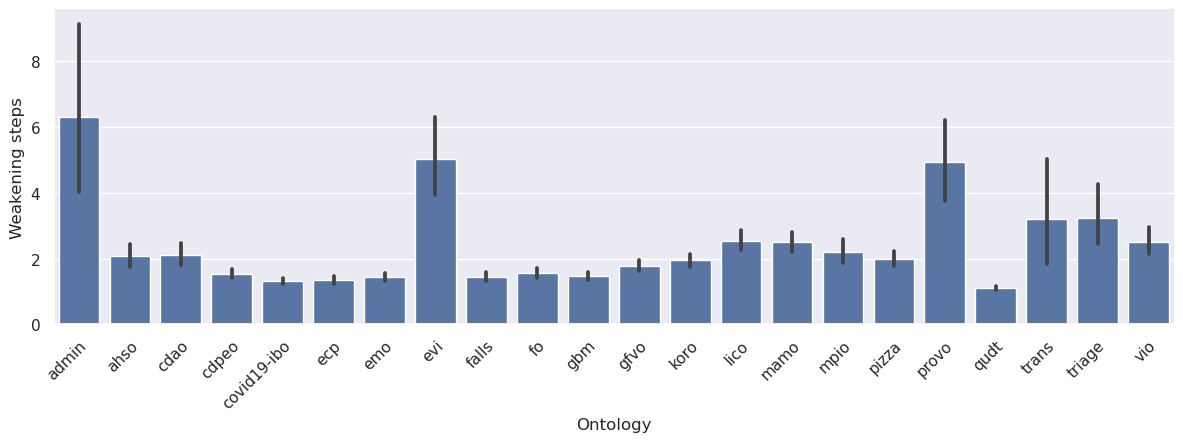
\includegraphics[width=\textwidth]{resources/steps-ontology-bar.png}
  \caption{Mean number of weakening steps needed for repairing the ontology. The error bars show the 95\% confidence interval.}
\end{figure}

\begin{figure}[ht]
  \centering
  \begin{subfigure}[T]{0.25\textwidth}
    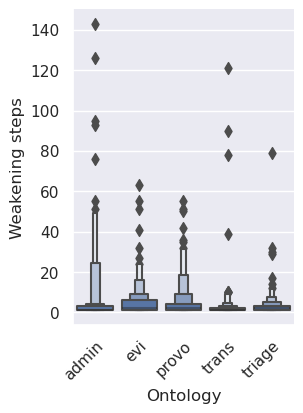
\includegraphics[width=\textwidth]{resources/steps-ontology-violin-1.png}
  \end{subfigure}
  \begin{subfigure}[T]{0.715\textwidth}
    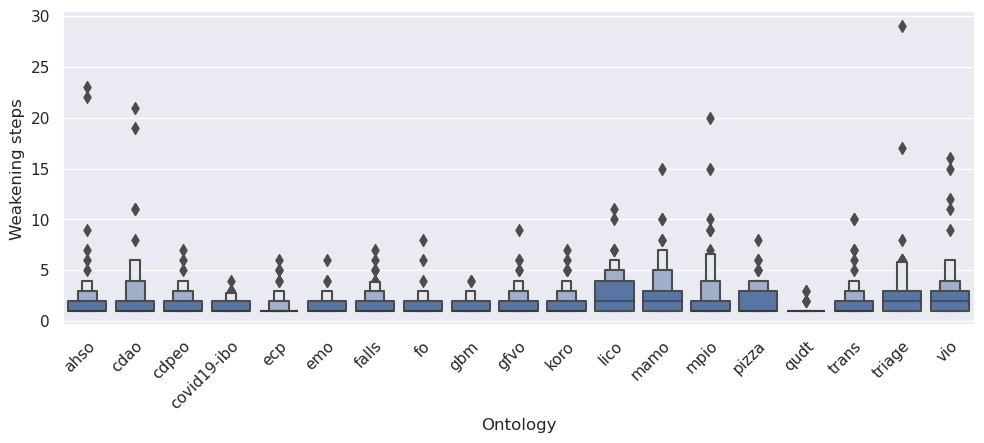
\includegraphics[width=\textwidth]{resources/steps-ontology-violin-2.png}
  \end{subfigure}
  \caption{Distribution of required weakening steps for repairing using axiom weakening by ontology. Attempts that failed by timeout were not considered.}
\end{figure}

\begin{figure}[ht]
  \centering
  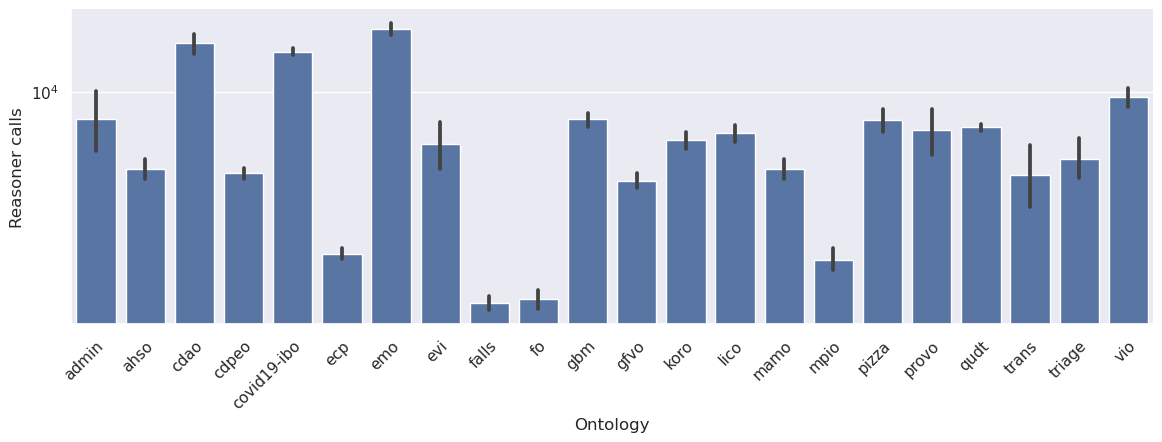
\includegraphics[width=\textwidth]{resources/calls-ontology-bar.png}
  \caption{Mean number of reasoner calls required for repairing using axiom weakening by ontology. The error bars show the 95\% confidence interval. Attempts that failed by timeout were not considered.}
\end{figure}

\begin{figure}[ht]
  \centering
  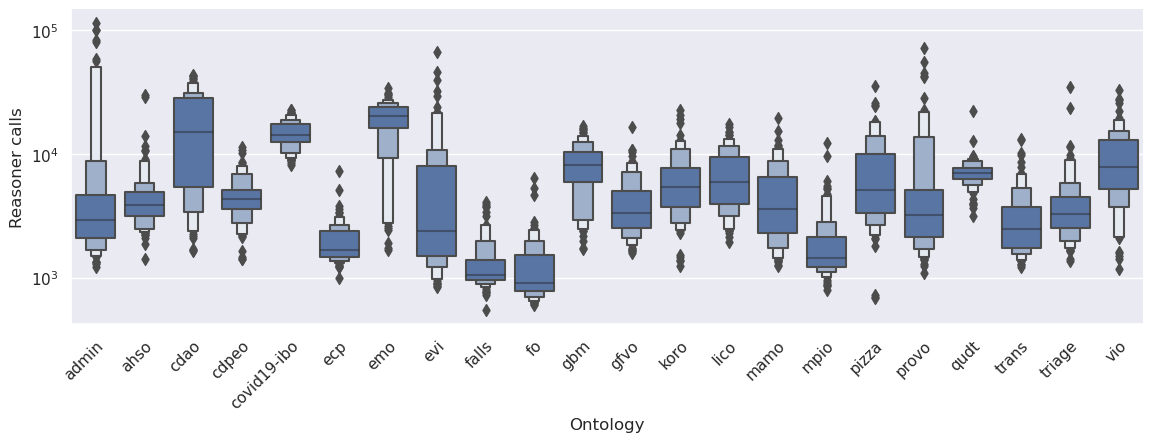
\includegraphics[width=\textwidth]{resources/calls-ontology-violin.png}
  \caption{Distribution of reasoner calls required for repairing using axiom weakening by ontology. Attempts that failed by timeout were not considered.}
\end{figure}

\begin{figure}[ht]
  \centering
  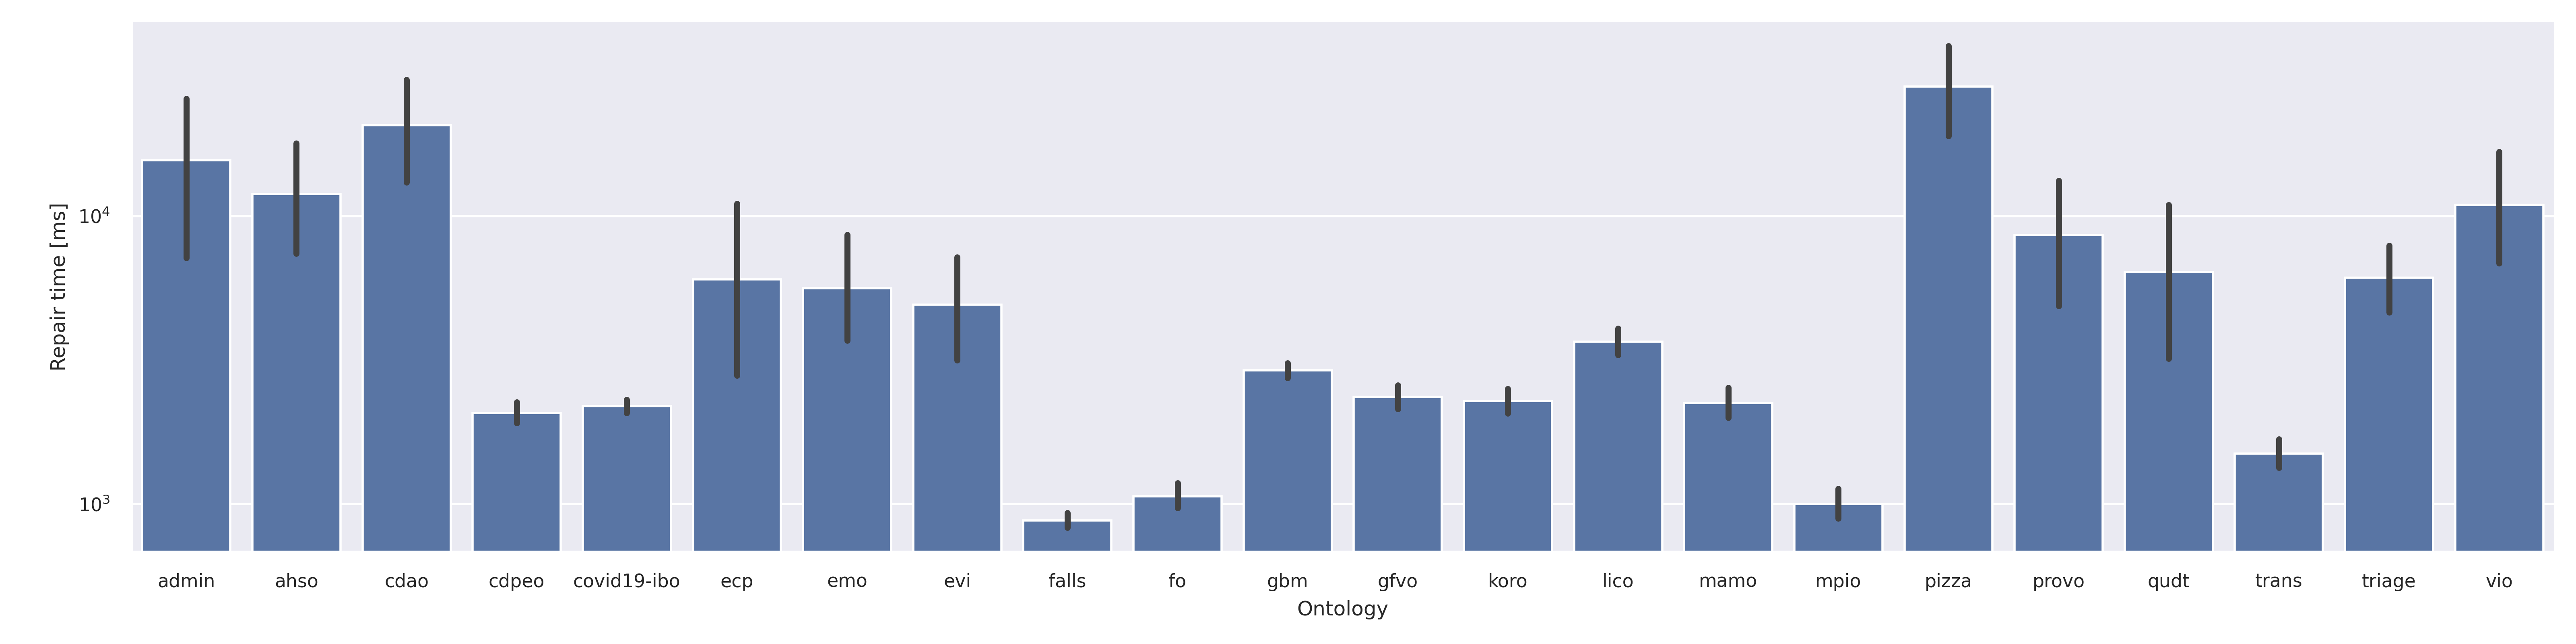
\includegraphics[width=\textwidth]{resources/time-ontology-bar.png}
  \caption{Mean execution time required for repairing using axiom weakening by ontology. The error bars show the 95\% confidence interval. Attempts that failed by timeout were not considered.}
\end{figure}

\begin{figure}[ht]
  \centering
  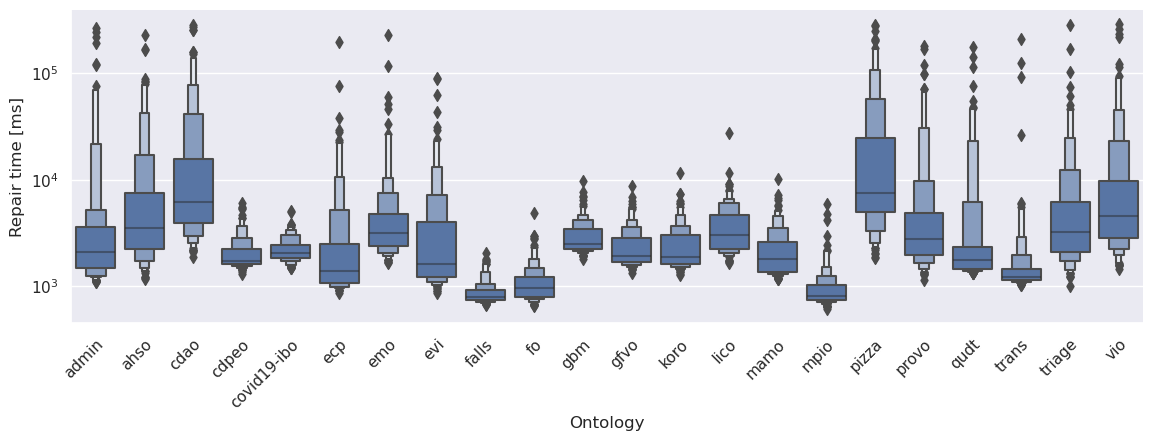
\includegraphics[width=\textwidth]{resources/time-ontology-violin.png}
  \caption{Distribution of execution time required for repairing using axiom weakening by ontology. Attempts that failed by timeout were not considered.}
\end{figure}

\begin{table}[ht]
  \scriptsize
  \centering
  \begin{tabular}{|l|r@{ }lr@{ }lr@{ }lr@{ }r|}
    \cline{2-9}
    \multicolumn{1}{l|}{} & \multicolumn{2}{c}{Steps} & \multicolumn{2}{c}{Calls} & \multicolumn{2}{c}{Time [ms]} & \multicolumn{2}{c|}{Failed} \\
    \hline
    admin & 13.3 & [4.3, 25.0] & 3199 & [2619, 3929] & 1834 & [1142, 2869] & 0\% & (2\%) \\
    ahso & 13.6 & [5.8, 25.2] & 3489 & [2981, 4136] & 12082 & [7920, 16710] & 2\% & (28\%) \\
    cdao & 3.9 & [2.9, 5.2] & 17109 & [15581, 18690] & 16868 & [12180, 22423] & 5\% & (51\%) \\
    cdpeo & 3.0 & [2.4, 4.0] & 4359 & [3903, 4850] & 1375 & [1283, 1525] & 0\% & (0\%) \\
    covid19-ibo & 2.1 & [1.8, 2.5] & 14377 & [13976, 14791] & 1698 & [1644, 1757] & 0\% & (13\%) \\
    ecp & 7.4 & [5.1, 10.0] & 1686 & [1435, 1975] & 2912 & [1840, 4494] & 1\% & (15\%) \\
    emo & 2.7 & [2.2, 3.3] & 19406 & [18699, 20060] & 7771 & [4859, 11450] & 0\% & (4\%) \\
    evi & 91.9 & [71.8, 114.0] & 5577 & [4316, 7016] & 6751 & [4733, 9214] & 1\% & (64\%) \\
    falls & 3.1 & [2.4, 4.0] & 812 & [700, 944] & 651 & [609, 701] & 0\% & (5\%) \\
    fo & 10.4 & [6.2, 16.1] & 1095 & [591, 1863] & 1358 & [820, 2235] & 4\% & (63\%) \\
    gbm & 3.5 & [2.8, 4.1] & 7726 & [7355, 8097] & 1793 & [1733, 1862] & 0\% & (0\%) \\
    gfvo & 10.3 & [7.6, 14.1] & 3155 & [2786, 3647] & 1527 & [1303, 1906] & 0\% & (0\%) \\
    koro & 5.6 & [4.6, 6.8] & 6353 & [5763, 7006] & 1406 & [1275, 1554] & 0\% & (0\%) \\
    lico & 10.7 & [8.6, 13.0] & 4671 & [4315, 5048] & 2438 & [2220, 2679] & 0\% & (22\%) \\
    mamo & 13.3 & [10.7, 15.9] & 2749 & [2505, 3001] & 1325 & [1237, 1423] & 0\% & (1\%) \\
    mpio & 4.2 & [3.5, 5.0] & 1055 & [1004, 1109] & 699 & [674, 727] & 0\% & (30\%) \\
    pizza & 28.4 & [21.3, 36.8] & 7180 & [6203, 8261] & 18099 & [13518, 23582] & 8\% & (59\%) \\
    provo & 35.2 & [27.1, 44.1] & 2860 & [2427, 3358] & 4831 & [3398, 6682] & 2\% & (9\%) \\
    qudt & 1.8 & [1.5, 2.1] & 6369 & [6183, 6569] & 5832 & [3533, 8749] & 1\% & (39\%) \\
    trans & 2.8 & [2.1, 3.6] & 2191 & [2035, 2356] & 1063 & [997, 1139] & 0\% & (5\%) \\
    triage & 34.0 & [23.0, 47.2] & 3186 & [2690, 3785] & 8790 & [5447, 12864] & 4\% & (53\%) \\
    vio & 10.5 & [7.4, 14.4] & 7101 & [6539, 7682] & 12995 & [8246, 18875] & 2\% & (8\%) \\
    \hline
  \end{tabular}
  \caption{Results of the evaluation with respect to performance while repairing using axiom weakening, but keeping the axioms of the reference ontology unchanged during repair. Number of weakening iterations, reasoner calls, and total repair time are given as sample mean, with 95\% confidence interval in brackets. The frequency of failed runs is shown as percentage of repairs by weakening that were started but not completed. In parentheses the percentage of total failed runs including those with timeout during generation of the inconsistent ontology. Note that repair using this method has only been attempted after the normal weakening based repair has been successful. This may skew the frequency of failures.}
\end{table}

\begin{figure}[ht]
  \centering
  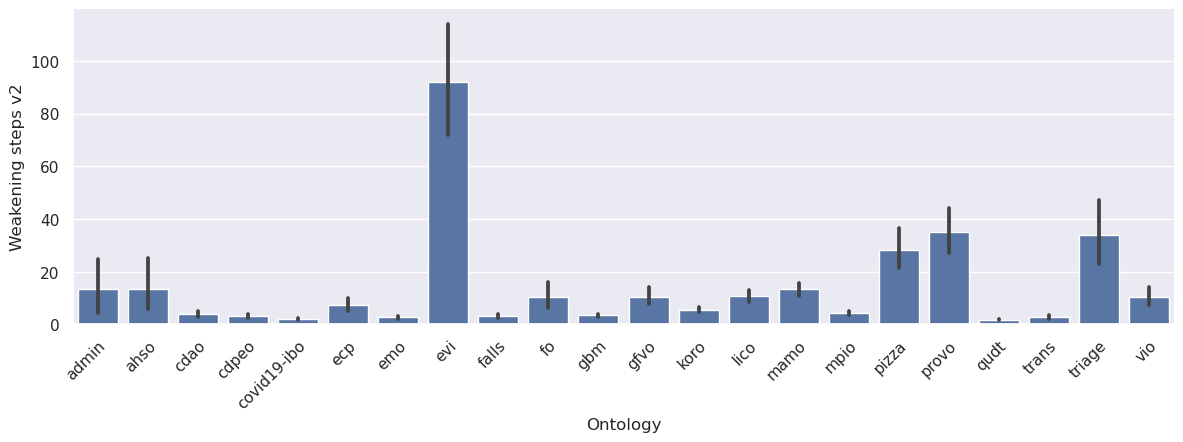
\includegraphics[width=\textwidth]{resources/steps-enhance-ontology-bar.png}
  \caption{Mean number of weakening steps needed for repairing the ontology (without weakening axioms in the reference ontology). The error bars show the 95\% confidence interval.}
\end{figure}

\begin{figure}[ht]
  \centering
  \begin{subfigure}[T]{0.25\textwidth}
    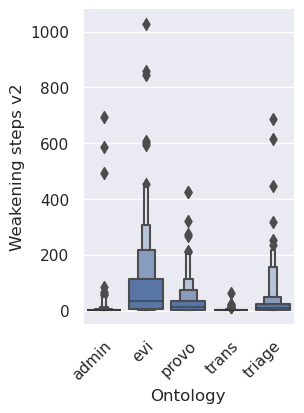
\includegraphics[width=\textwidth]{resources/steps-enhance-ontology-violin-1.png}
  \end{subfigure}
  \begin{subfigure}[T]{0.715\textwidth}
    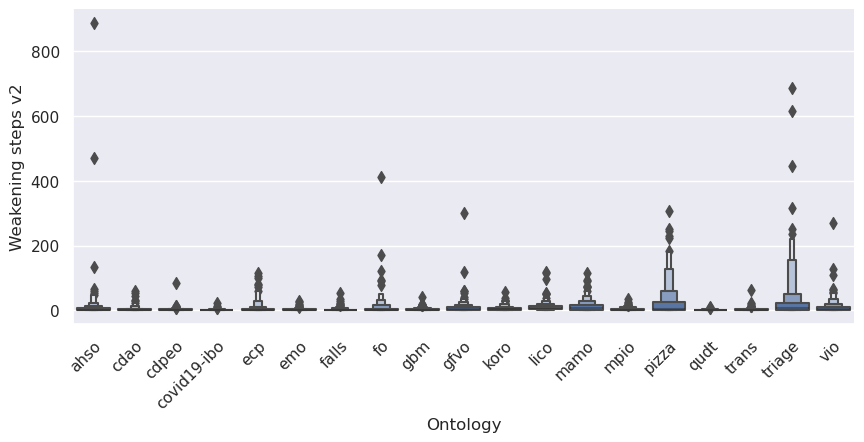
\includegraphics[width=\textwidth]{resources/steps-enhance-ontology-violin-2.png}
  \end{subfigure}
  \caption{Distribution of required weakening steps for repairing using axiom weakening (without weakening axioms in the reference ontology) by ontology. Attempts that failed by timeout were not considered.}
\end{figure}

\begin{figure}[ht]
  \centering
  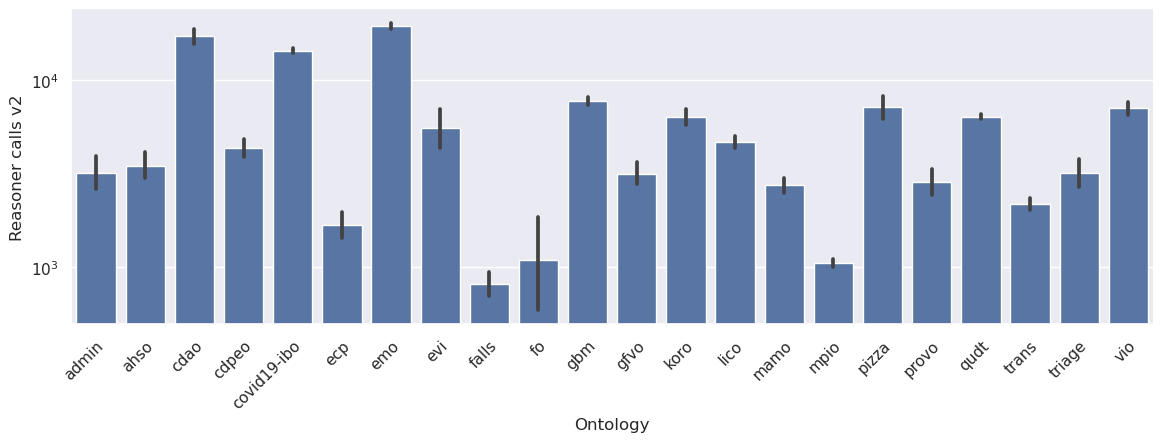
\includegraphics[width=\textwidth]{resources/calls-enhance-ontology-bar.png}
  \caption{Mean number of reasoner calls required for repairing using axiom weakening (without weakening axioms in the reference ontology) by ontology. The error bars show the 95\% confidence interval. Attempts that failed by timeout were not considered.}
\end{figure}

\begin{figure}[ht]
  \centering
  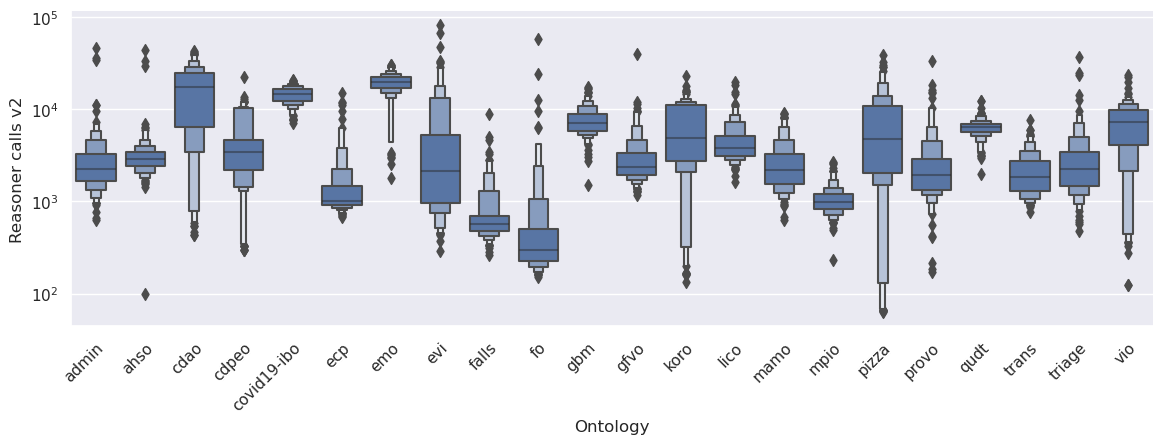
\includegraphics[width=\textwidth]{resources/calls-enhance-ontology-violin.png}
  \caption{Distribution of reasoner calls required for repairing using axiom weakening (without weakening axioms in the reference ontology) by ontology. Attempts that failed by timeout were not considered.}
\end{figure}

\begin{figure}[ht]
  \centering
  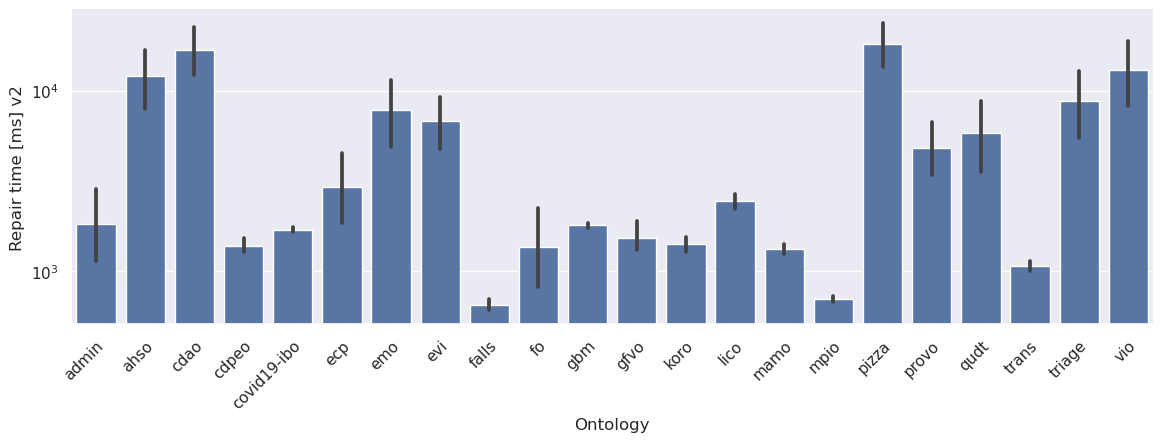
\includegraphics[width=\textwidth]{resources/time-enhance-ontology-bar.png}
  \caption{Mean execution time required for repairing using axiom weakening (without weakening axioms in the reference ontology) by ontology. The error bars show the 95\% confidence interval. Attempts that failed by timeout were not considered.}
\end{figure}

\begin{figure}[ht]
  \centering
  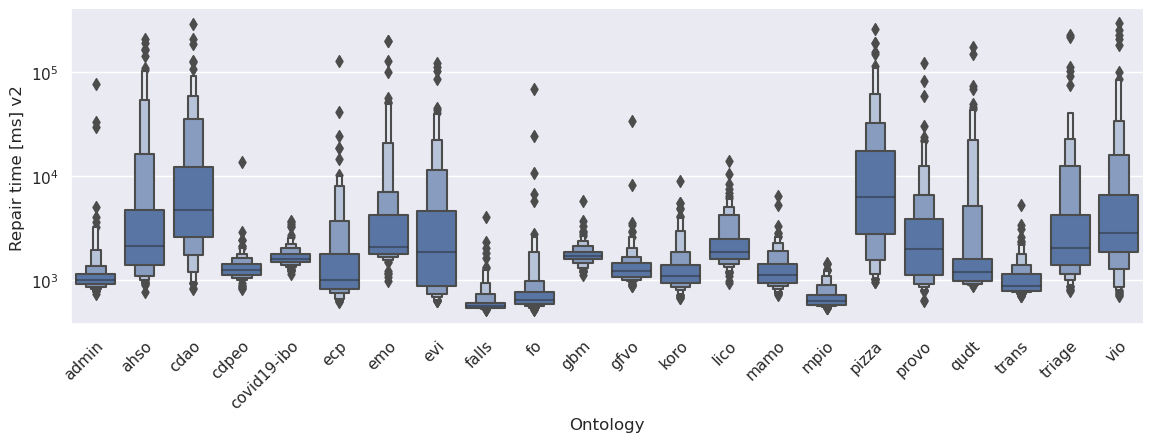
\includegraphics[width=\textwidth]{resources/time-enhance-ontology-violin.png}
  \caption{Distribution of execution time required for repairing using axiom weakening (without weakening axioms in the reference ontology) by ontology. Attempts that failed by timeout were not considered.}
\end{figure}

